% ========================================
% Document Metadata
% ========================================
% Working number: #61
% DOI: 10.5281/zenodo.19934138
% This paper reports a striking coincidence: a quark-scale mass emerges
% directly from the empirical anomalous magnetic moment of the proton.

% ========================================
% Document Class and Package Setup
% ========================================
\documentclass[%
 reprint, amsmath,amssymb, aps, prc, ]{revtex4-2}

% Basic packages
\usepackage{graphicx}
\usepackage{bm}

% Quantum mechanics notation
\usepackage{physics}

% Hyperlinks
\usepackage[colorlinks=true,
            linkcolor=blue, filecolor=blue, urlcolor=blue, citecolor=blue]{hyperref}

% Caption setup
\usepackage{caption}
\captionsetup[figure]{
    justification=raggedright, labelfont={bf}, name={Fig.}, labelsep=period }
\captionsetup[table]{
    labelfont={bf}, name={Table}, labelsep=period }

% Equation numbering per section
\numberwithin{equation}{section}

% ========================================
% Typography Configuration
% ========================================
\tolerance=1000
\emergencystretch=1em
\hyphenpenalty=3000
\exhyphenpenalty=3000
\flushbottom

% ========================================
% Microtype and Additional Packages
% ========================================
\usepackage[final]{microtype}
\usepackage{ragged2e}
\usepackage{booktabs}
\usepackage{enumitem}

% ========================================
% Theorem Environment
% ========================================
\usepackage{amsthm}
\newtheorem{theorem}{Theorem}[section]

% ========================================
% TikZ for Appendix Schematic Figure
% ========================================
\usepackage{tikz}
\usetikzlibrary{arrows.meta, calc, positioning}

% ========================================
% Custom Commands: Internal Phase Notation
% ========================================
\newcommand{\iphase}{\theta}
\newcommand{\omZB}{\omega_{\text{ZB}}}
\newcommand{\vZB}{v_{\text{ZB}}}

% ========================================
% Document Begin
% ========================================
\begin{document}

% ========================================
% Title, Author, and Date
% ========================================
\title{Application of the $\gamma$-Equation to the Proton:\\
A Parameter-Free Hadronic Mass Scale}

\author{Satoshi Hanamura}
\email{hana.tensor@gmail.com}
\date{June 6, 2026}

% ========================================
% Abstract
% ========================================
\begin{abstract}
The bridge equation $\gamma = 1 + |a|$, originally derived in the 0-Sphere model from a first-principles geometric argument relating the anomalous magnetic moment $a$ of a spin-$1/2$ particle to the Lorentz factor of an internal Zitterbewegung oscillation, determines the kernel rest mass through the relativistic relation between the rest-frame and externally observed mass.
The internal Zitterbewegung velocity is obtained instead through the velocity-determining Lorentz factor $\gamma_v = 1 + |a|/\sqrt{2}$, in which the anomalous moment enters through its root-mean-square value; this reduction is established machinery of the model.
For the electron, $\gamma_v$ reproduces the established 0-Sphere prediction $\vZB^e \approx 0.04\,c$ from the empirical value $a_e \approx 1.16 \times 10^{-3}$.
The first-principles geometric origin of the equation does not depend on perturbative expansion and remains formally well-defined when $a$ is large.
We apply the equation directly to the proton, using the empirical proton anomalous magnetic moment $a_p \approx 1.793$ and the proton mass $m_p \approx 938.27 \text{ MeV}/c^2$.
The resulting mass-determining Lorentz factor is $\gamma_p \approx 2.793$ and the velocity-determining Lorentz factor is $\gamma_{v,p} \approx 2.268$; the predicted internal Zitterbewegung velocity is $\vZB^p \approx 0.898\,c$, and the inferred kernel rest mass of the proton is $m_{0}^{p} = m_p / \gamma_p \approx 336 \text{ MeV}/c^2$.
This kernel rest mass falls within the empirically established constituent quark mass band of approximately $300\text{--}350$ MeV$/c^2$ for the up and down quarks, derived in QCD-based descriptions of the nucleon through chiral symmetry breaking phenomenology and baryon spectroscopy fits, and coincides numerically with the frequently cited benchmark value of $336$ MeV$/c^2$ within this band.
The 0-Sphere prediction is determined parameter-free by the empirical inputs $\{m_p, a_p\}$ via the bridge equation; no parameter is fit to QCD spectroscopic data at any stage of the derivation.
The two routes use operationally independent empirical inputs and structurally distinct intermediate machinery (the Lorentz factor of internal kernel oscillation versus dynamical mass generation through chiral symmetry breaking).
We interpret this consistency as an empirical anchor for the 0-Sphere framework at the hadronic mass scale, suggesting that the 0-Sphere kernel rest mass and the QCD constituent quark mass scale describe the same underlying effective hadronic mass scale through different theoretical descriptions.
The effective Compton wavelength implied by $m_0^p$ is $\bar{\lambda}_C^{\text{kernel}} \approx 0.59$ fm, comparable to the proton charge radius and consistent with hadronic confinement scales, providing an internal consistency check.
Stress tests, defensive elaborations, and the geometric origin of the hadronic mass scale are identified as directions for future work.
\end{abstract}

\maketitle

% ========================================
% Section 1: Introduction
% ========================================
\section{Introduction}

The 0-Sphere model, developed by the present author across a series of papers since 2018 \cite{Hanamura1}, articulates a geometric structure for charged spin-$1/2$ particles in which the rest mass of the particle is generated by an internal oscillation between two thermal-potential-energy kernels separated at the Compton scale.
A central result of this program, derived in \cite{Hanamura10}, is the bridge equation
\begin{equation}
\gamma \;=\; 1 + |a|,
\label{eq:bridge}
\end{equation}
relating the Lorentz factor $\gamma$ of the internal kernel oscillation to the empirical anomalous magnetic moment $a$ of the particle.
This mass-determining Lorentz factor governs the relativistic relation between the rest-frame energy of the kernel and the externally observed mass of the particle.
The internal Zitterbewegung velocity is obtained instead from the velocity-determining Lorentz factor
\begin{equation}
\gamma_v \;=\; 1 + \frac{|a|}{\sqrt{2}},
\label{eq:gammav}
\end{equation}
in which the anomalous moment enters through its root-mean-square value $|a|/\sqrt{2}$, the standard peak-to-root-mean-square reduction of a sinusoidal quantity.
The structural distinction between the two Lorentz factors is developed in Section~\ref{sec:gammaeq}.
For the electron, where $a_e \approx 1.16 \times 10^{-3}$, equations~\eqref{eq:bridge} and~\eqref{eq:gammav} give
\begin{equation}
\frac{\vZB^e}{c} \;=\; \sqrt{1 - \frac{1}{\gamma_{v,e}^{2}}} \;\approx\; 0.04047,
\label{eq:vZBe}
\end{equation}
placing the electron's internal oscillation in the non-relativistic regime $\gamma_{v,e} \approx 1.0008$.
This value is not a new prediction of the present paper. The electron internal Zitterbewegung velocity $\vZB^e \approx 0.04\,c$ is the foundational numerical signature of the 0-Sphere model, established in~\cite{Hanamura10} and serving since then as the central falsifiable prediction of the electron sector. The present treatment recovers it as the velocity-determining Lorentz factor applied to the electron; the contribution of the present paper is the extension of the same construction to the proton.

The geometric argument used in \cite{Hanamura10} to derive equation~\eqref{eq:bridge} does not invoke perturbation theory at any stage.
This is in contrast to the standard QED calculation of $a_e$, which is constructed as an asymptotic series in the fine-structure constant $\alpha$ and matches experiment to extraordinary precision precisely \emph{because} the electron is well within the perturbative regime.
For the proton, however, the situation is structurally different.
The proton anomalous magnetic moment $a_p \approx 1.793$ is approximately $1500$ times larger than $a_e$, and perturbative QCD breaks down entirely at the relevant scale.
The standard treatment of $a_p$ within the Standard Model is therefore not a perturbative calculation but a phenomenological extraction from low-energy hadronic data, supplemented by lattice QCD calculations and constituent quark model fits.

This raises the central question of the present paper.
The bridge equation~\eqref{eq:bridge} was derived without recourse to perturbation theory.
There is therefore no formal obstruction to applying it directly to the proton, even though perturbative QED methods would fail there.
What does the equation predict in this regime, and is the prediction empirically meaningful?

The result, derived below, is non-trivial.
The kernel rest mass inferred from~\eqref{eq:bridge} applied to the proton falls within the empirically established constituent quark mass band of QCD-based nucleon descriptions and coincides with the frequently cited $336$ MeV$/c^2$ benchmark in the constituent quark model literature, despite the two routes using disjoint empirical inputs and structurally distinct intermediate machinery.
We interpret this consistency as an empirical anchor for the 0-Sphere framework at the hadronic scale.

The scope of the present paper is deliberately restricted to this two-framework comparison and its immediate internal consistency checks.
The extension of equation~\eqref{eq:bridge} to other spin-$1/2$ particles and the geometric origin of the hadronic mass scale are separately substantial topics identified as future work.
Section~\ref{sec:gammaeq} recalls the derivation of equation~\eqref{eq:bridge} and its application to the electron in concise form.
Section~\ref{sec:proton} presents the application to the proton.
Section~\ref{sec:qcd} compares the resulting kernel rest mass with the QCD constituent quark mass scale and articulates the epistemological status of the comparison.
Section~\ref{sec:compton} provides the effective Compton wavelength internal consistency check.
Section~\ref{sec:discussion} discusses the falsifiability profile and the relation to the broader 0-Sphere program.
Section~\ref{sec:open} catalogues the open problems explicitly deferred from the present scope.
Section~\ref{sec:conclusion} concludes.

\begin{table*}[t!]
\centering
\caption{\textbf{Kinematic regime comparison: electron vs proton via the $\gamma$-equation}}
\label{tab:e_vs_p}
\renewcommand{\arraystretch}{1.4}
\begin{tabular}{p{2.3cm}p{2.3cm}p{2.7cm}p{2.7cm}p{2.0cm}p{2.6cm}}
\toprule
\textbf{Particle} & \textbf{$|a|$} & \textbf{$\gamma = 1+|a|$ (mass)} & \textbf{$\gamma_v = 1+|a|/\sqrt{2}$ (velocity)} & \textbf{$\vZB / c$} & \textbf{Regime} \\
\midrule
Electron
& $1.16 \times 10^{-3}$
& $1.00116$
& $1.00082$
& $0.04047$
& non-relativistic \\
\addlinespace[0.3cm]
Proton
& $1.7928$
& $2.7928$
& $2.2677$
& $0.898$
& highly relativistic \\
\addlinespace[0.2cm]
\bottomrule
\end{tabular}
\vspace{0.2cm}
\begin{minipage}{0.95\textwidth}
\justifying\footnotesize
Empirical values of $a$ taken from the Particle Data Group compilation~\cite{PDG}.
The mass-determining Lorentz factor $\gamma = 1 + |a|$ follows from the bridge equation~\eqref{eq:bridge} of \cite{Hanamura10} and fixes the kernel rest mass through $m_0 = m/\gamma$.
The velocity-determining Lorentz factor $\gamma_v = 1 + |a|/\sqrt{2}$ uses the effective (root-mean-square) value of the anomalous moment and fixes the internal Zitterbewegung velocity through $\vZB / c = \sqrt{1 - 1/\gamma_v^2}$.
The qualitative regime label distinguishes the non-relativistic electron case ($\gamma$ and $\gamma_v$ both within parts-per-thousand of unity) from the highly relativistic proton case (near-luminal internal motion).
\end{minipage}
\end{table*}

% ========================================
% Section 2: The Gamma-Equation Recapped
% ========================================
\section{The $\gamma$-Equation Recapped}
\label{sec:gammaeq}

The 0-Sphere model treats a spin-$1/2$ particle as a composite of two thermal-potential-energy kernels separated by a distance of order the Compton wavelength and oscillating with frequency $\omZB$ characteristic of Zitterbewegung, the rapid internal oscillation arising in the Dirac equation~\cite{Dirac1928} from the interference of positive- and negative-energy components~\cite{Schrodinger1930}.
The rest mass of the particle in this picture is not a primitive parameter but an emergent quantity, set by the time-averaged thermal-potential-energy content of the kernel pair.
The internal oscillation contributes an effective Lorentz factor to the relation between the rest-frame energy of the kernel and the externally observed mass of the particle.
The detailed geometric derivation, which we do not reproduce here, is given in~\cite{Hanamura10}.
The result is the bridge equation~\eqref{eq:bridge} relating the empirically measured anomalous magnetic moment $a$ to the Lorentz factor $\gamma$ of the internal oscillation.

Two quantities are extracted from the internal oscillation through two distinct Lorentz factors, and the distinction between them is a structural feature of the framework, not an auxiliary assumption of the present paper. The kernel rest mass couples to the anomalous moment through the mass-determining Lorentz factor $\gamma = 1 + |a|$ of equation~\eqref{eq:bridge}, and is obtained as $m_0 = m/\gamma$. The internal Zitterbewegung velocity is obtained instead from the velocity-determining Lorentz factor $\gamma_v = 1 + |a|/\sqrt{2}$ of equation~\eqref{eq:gammav}; the velocity is then $\vZB/c = \sqrt{1 - 1/\gamma_v^2}$. The two factors differ because they refer to two physically distinct features of one and the same oscillation. The anomalous magnetic moment $a$ measures the peak Lorentz contraction---the contraction at the instant of maximum internal velocity---and the mass-determining factor $\gamma = 1 + |a|$ uses this peak quantity directly. The internal Zitterbewegung velocity, by contrast, is an ongoing oscillation whose physically representative value is its time average; the time-averaged (root-mean-square) velocity is obtained from the peak through the standard sinusoidal ratio $X_{\text{rms}} = X_{\text{peak}}/\sqrt{2}$, which is why the velocity-determining factor carries the reduced value $|a|/\sqrt{2}$. This root-mean-square reduction is established machinery of the 0-Sphere model: it was introduced in the foundational treatment~\cite{Hanamura10} and set out in detail in~\cite{Hanamura11,Hanamura14}, where the velocity-determining relation $L/L_0 = 1/(1+|a|/\sqrt{2})$ is given explicitly on the stated ground that the time-averaged, rather than the peak, internal velocity is sought, and the electron internal velocity $\vZB^e \approx 0.04\,c$---the central falsifiable signature of the framework---is derived from the root-mean-square-corrected relation rather than from the peak relation. The distinction has negligible numerical consequence for the electron, where $|a|$ is small and $\gamma$ and $\gamma_v$ differ only at the $10^{-4}$ level, but becomes significant for the proton, where $|a|$ is of order unity and the two Lorentz factors differ substantially. The present paper therefore does not introduce the $\sqrt{2}$ factor; it applies the mass-determining and velocity-determining factors, both already part of the framework, to the proton. The first-principles origin of the factor $1/\sqrt{2}$---that it is the square root of the average-to-peak ratio of the momentum term $\tfrac{1}{2}\sin^2\theta$ in the conservation identity, rather than an imported sinusoidal-average analogy---lies outside the scope of the present paper, which uses the velocity-determining factor as established machinery of the framework.

For the electron, the empirical value $a_e \approx 1.16 \times 10^{-3}$~\cite{PDG} produces a mass-determining Lorentz factor $\gamma_e \approx 1.00116$ and a velocity-determining Lorentz factor $\gamma_{v,e} \approx 1.00082$, hence the internal Zitterbewegung velocity given in~\eqref{eq:vZBe}.
The kernel rest mass of the electron is then
\begin{equation}
m_{0}^{e} \;=\; \frac{m_e}{\gamma_e} \;\approx\; \frac{0.511 \text{ MeV}/c^2}{1.00116} \;\approx\; 0.510 \text{ MeV}/c^2,
\label{eq:m0e}
\end{equation}
indistinguishable from the observed electron mass at the precision relevant here.
This is consistent with the standard reading of the electron as an elementary particle: the kernel oscillation is non-relativistic, the rest mass and the kernel rest mass differ only at the part-per-thousand level, and no internal substructure beyond the kernel pair is inferred.

The non-perturbative character of the derivation in~\cite{Hanamura10} bears emphasis.
The geometric argument identifies $\gamma$ with the Lorentz factor of an internal motion whose existence is an ontological commitment of the 0-Sphere framework, not a mathematical artifact of an expansion.
The right-hand side of~\eqref{eq:bridge} is the empirical anomalous magnetic moment, taken without modification from experiment.
Neither side of the equation contains a parameter that becomes meaningless or singular when $a$ is large.
This formal robustness is what permits, in the next section, the direct application of the equation to a regime in which standard perturbative methods break down entirely.

% ========================================
% Section 3: Application to the Proton
% ========================================
\section{Application to the Proton}
\label{sec:proton}

The empirical inputs for the application to the proton are the proton mass and the proton anomalous magnetic moment, both well-determined experimental quantities.
We use the values
\begin{align}
m_p &\;=\; 938.272 \text{ MeV}/c^2,\label{eq:mp}\\
a_p &\;=\; 1.7928,\label{eq:ap}
\end{align}
taken from the most recent compilation of the Particle Data Group~\cite{PDG}.
The latter value follows from the proton's $g$-factor $g_p \approx 5.586$ via the standard definition $a_p = (g_p - 2)/2$.

Direct substitution into the bridge equation~\eqref{eq:bridge} yields the mass-determining Lorentz factor
\begin{equation}
\gamma_p \;=\; 1 + |a_p| \;=\; 2.7928,
\label{eq:gammap}
\end{equation}
while the velocity-determining Lorentz factor of equation~\eqref{eq:gammav} is
\begin{equation}
\gamma_{v,p} \;=\; 1 + \frac{|a_p|}{\sqrt{2}} \;=\; 2.2677.
\label{eq:gammavp}
\end{equation}
The predicted internal Zitterbewegung velocity of the proton kernel oscillation follows from the velocity-determining Lorentz factor through the standard relativistic relation
\begin{equation}
\frac{\vZB^p}{c} \;=\; \sqrt{1 - \frac{1}{\gamma_{v,p}^{2}}} \;=\; \sqrt{1 - \frac{1}{(2.2677)^2}} \;\approx\; 0.898.
\label{eq:vZBp}
\end{equation}
The proton's internal kernel oscillation is therefore predicted to be highly relativistic, with $\vZB^p \approx 0.898\,c$, in stark contrast to the non-relativistic regime of the electron.

The kernel rest mass of the proton is then determined by the standard relativistic energy-mass relation between the rest frame of the kernel oscillator and the externally observed proton mass,
\begin{equation}
m_{0}^{p} \;=\; \frac{m_p}{\gamma_p} \;=\; \frac{938.272 \text{ MeV}/c^2}{2.7928} \;\approx\; 335.94 \text{ MeV}/c^2.
\label{eq:m0p}
\end{equation}
We round this to $m_0^p \approx 336 \text{ MeV}/c^2$ for subsequent comparison.

Equation~\eqref{eq:m0p} carries a specific physical interpretation.
It states that the rest mass of the kernel oscillator inside the proton, in the rest frame of the kernel itself, is approximately $336$ MeV$/c^2$, considerably less than the proton's externally observed mass of $938.27$ MeV$/c^2$.
The factor between these two values, the mass-determining Lorentz factor $\gamma_p = 2.7928$, is supplied by the relativistic enhancement associated with the internal kernel motion.
In the language of relativistic kinematics, the observed proton mass corresponds to the total energy associated with the relativistically oscillating kernel degree of freedom, related to the kernel's proper-frame rest energy by the Lorentz factor of the internal motion.
This is the same relation that governs the electron in equation~\eqref{eq:m0e}, with the only difference being the magnitude of $\gamma$.
For the electron, $\gamma$ is so close to unity that the kernel rest mass and the observed mass are numerically indistinguishable.
For the proton, $\gamma$ is large enough that the two differ by nearly a factor of three.

The full derivation chain may be summarized compactly as
\begin{align}
\{m_p,\, a_p\}
&\;\xrightarrow{\;\gamma = 1+|a|\;}\; \gamma_p
\notag\\
&\;\xrightarrow{\;m_0 = m/\gamma\;}\; m_0^p \;\approx\; 335.94 \text{ MeV}/c^2,
\label{eq:derivation-chain}
\end{align}
with no free parameter at any stage.

A summary of the kinematic regime contrast between the two particles is provided in Table~\ref{tab:e_vs_p}.

The bridge equation thus exhibits a qualitative regime bifurcation between the two particles: a single framework, applied without modification, places the electron in the near-non-relativistic internal regime and the proton in the strongly relativistic internal regime. The empirical anomalous magnetic moment $|a|$ is the sole quantity that drives this transition, entering both the mass-determining factor $\gamma = 1+|a|$ and the velocity-determining factor $\gamma_v = 1+|a|/\sqrt{2}$, and the difference between the two cases is encoded entirely in its magnitude. This regime structure is the mechanism by which the non-perturbatively derived bridge equation can address the hadronic regime where standard perturbative techniques fail; the subsequent comparison with the constituent quark mass scale in Section~\ref{sec:qcd} is the empirical anchor that gives this regime extension testable physical content.


\begin{figure*}[t!]
\centering
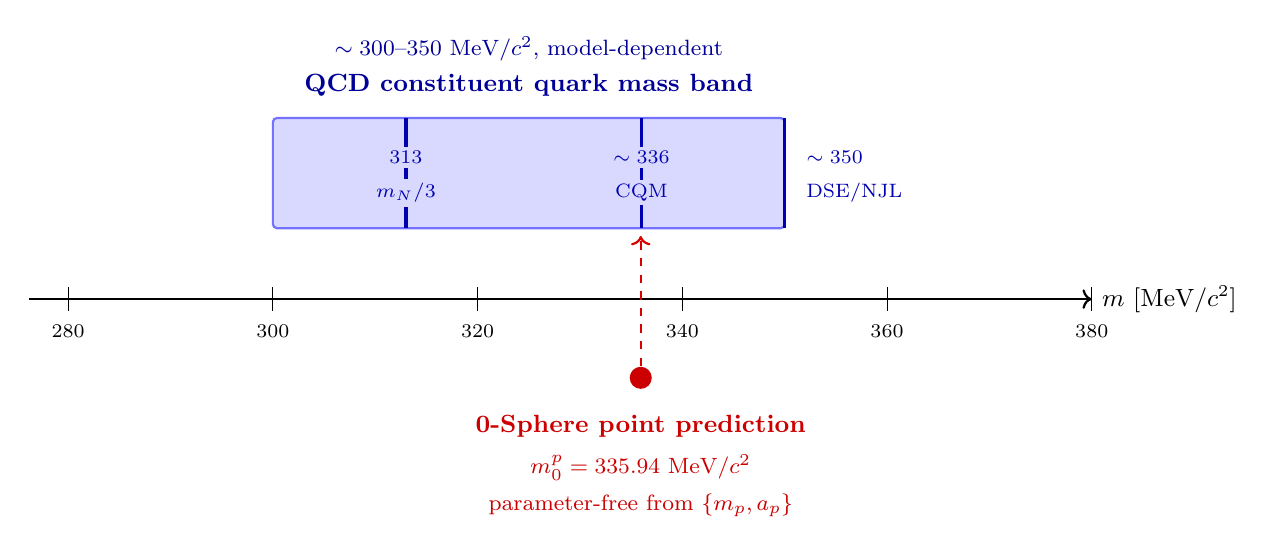
\begin{tikzpicture}[x=1mm, y=1mm]
% Mass axis (1 MeV = 1.3 mm scaling; m=280 -> x=10, m=380 -> x=140)
\draw[->, thick] (5,0) -- (140,0) node[right, font=\small] {$m\ [\text{MeV}/c^2]$};
% Tick marks below axis
\foreach \x/\xlabel in {10/280, 36/300, 62/320, 88/340, 114/360, 140/380} {
  \draw (\x,-1.5) -- (\x,1.5);
  \node[below, font=\scriptsize, anchor=north] at (\x,-2) {\xlabel};
}
% QCD band shaded region (300-350 MeV) -> x=36 to x=101
\fill[blue!15, rounded corners=1.5pt] (36,9) rectangle (101,23);
\draw[blue!55, thick, rounded corners=1.5pt] (36,9) rectangle (101,23);
% Band labels above band
\node[blue!60!black, font=\small\bfseries, anchor=south] at (68.5,24.5)
  {QCD constituent quark mass band};
\node[blue!60!black, font=\footnotesize, anchor=south] at (68.5,29)
  {$\sim 300\text{--}350$ MeV$/c^2$, model-dependent};
% Benchmark vertical markers (full band height; m=313 -> x=52.9, m=336 -> x=82.8, m=350 -> x=101)
\draw[blue!70!black, very thick] (52.9,9) -- (52.9,23);
\draw[blue!70!black, very thick] (82.8,9) -- (82.8,23);
\draw[blue!70!black, very thick] (101,9) -- (101,23);
% Benchmark labels with band-colored fill (interrupts vertical lines visually)
\node[blue!70!black, font=\scriptsize, fill=blue!15, inner sep=1.5pt, anchor=center] at (52.9,18) {$313$};
\node[blue!70!black, font=\scriptsize, fill=blue!15, inner sep=1.5pt, anchor=center] at (52.9,13.5) {$m_N/3$};
\node[blue!70!black, font=\scriptsize, fill=blue!15, inner sep=1.5pt, anchor=center] at (82.8,18) {$\sim 336$};
\node[blue!70!black, font=\scriptsize, fill=blue!15, inner sep=1.5pt, anchor=center] at (82.8,13.5) {CQM};
% 350 label outside band right edge (no fill needed since outside band)
\node[blue!70!black, font=\scriptsize, anchor=west] at (102.5,18) {$\sim 350$};
\node[blue!70!black, font=\scriptsize, anchor=west] at (102.5,13.5) {DSE/NJL};
% 0-Sphere point prediction (red, below axis at m=335.94 -> x=82.722)
\fill[red!80!black] (82.72,-10) circle (1.4);
\draw[->, red!85!black, thick, dashed] (82.72,-8.5) -- (82.72,8);
\node[red!80!black, font=\small\bfseries, anchor=north] at (82.72,-13.5)
  {0-Sphere point prediction};
\node[red!80!black, font=\footnotesize, anchor=north] at (82.72,-18.5)
  {$m_0^p = 335.94$ MeV$/c^2$};
\node[red!80!black, font=\footnotesize, anchor=north] at (82.72,-23.5)
  {parameter-free from $\{m_p, a_p\}$};
\end{tikzpicture}
\caption{\textbf{QCD constituent quark mass band versus the 0-Sphere point prediction}}
\label{fig:band_vs_point}
\vspace{0.4em}
\begin{minipage}{0.95\textwidth}
\justifying\small
Schematic representation of the asymmetry between the QCD constituent quark mass band and the 0-Sphere point prediction. The QCD band (shaded blue, $\sim 300\text{--}350$ MeV$/c^2$) contains common benchmark values: $313$ MeV$/c^2$ from the naive equipartition $m_N/3$, approximately $336$ MeV$/c^2$ from constituent quark model spectroscopic fits, and approximately $350$ MeV$/c^2$ in Dyson--Schwinger and Nambu--Jona-Lasinio analyses. The 0-Sphere prediction (red, below the axis) is determined parameter-free from the empirical inputs $\{m_p, a_p\}$ via the bridge equation $\gamma = 1 + |a|$ and lands within the band near the constituent quark model benchmark. The two routes use disjoint input data and disjoint intermediate machinery; the compatibility of their outputs is the empirical anchor reported in this work.
\end{minipage}
\end{figure*}

% ========================================
% Section 4: Comparison with the Constituent Quark Mass Scale
% ========================================
\section{Comparison with the Constituent Quark Mass Scale}
\label{sec:qcd}

The kernel rest mass of the proton, equation~\eqref{eq:m0p}, takes the value $m_0^p \approx 335.94$ MeV$/c^2$ from the empirical inputs $m_p$ and $a_p$.
A structurally analogous mass scale arises in QCD-based descriptions of the nucleon through chiral symmetry breaking phenomenology and constituent quark model fits.
We summarize that scale and compare it with the 0-Sphere prediction.

In the QCD Lagrangian, the up and down quarks carry small bare masses, the so-called current quark masses, with empirical values $m_u \approx 2.2 \text{ MeV}/c^2$ and $m_d \approx 4.7 \text{ MeV}/c^2$~\cite{PDG}.
These bare values cannot account for the proton mass of $938.27 \text{ MeV}/c^2$, which exceeds the sum of three bare quarks by more than two orders of magnitude.
The accepted resolution within QCD is that the chiral symmetry of the massless-quark Lagrangian is broken spontaneously by a non-vanishing quark-antiquark vacuum condensate, $\langle \bar{q} q \rangle \neq 0$, which dynamically endows the quark with an effective mass much larger than its bare current mass at hadronic scales~\cite{HalzenMartin,Griffiths}.
The resulting dynamical mass is conventionally termed the constituent quark mass.

We emphasize at the outset that the constituent quark mass is not a sharply defined physical constant analogous to the electron mass.
It is a scale-, gauge-, and model-dependent effective parameter, extracted in low-energy hadronic environments through specific model fits and not directly computable from the QCD Lagrangian as a closed-form quantity.
The empirical band cited for the up and down quarks in the constituent quark model literature is approximately
\begin{equation}
m_q^{\text{const}} \;\approx\; 300\text{--}350 \text{ MeV}/c^2,
\label{eq:mconst_band}
\end{equation}
with specific benchmark values within this band depending on the choice of model and the spectroscopic data used in the fit.
Common benchmarks include $313 \text{ MeV}/c^2$ obtained from the naive equipartition $m_N / 3 \approx 938/3$, approximately $336 \text{ MeV}/c^2$ from constituent quark model fits to baryon and meson spectroscopy, and values up to approximately $350 \text{ MeV}/c^2$ in certain Nambu--Jona-Lasinio fits and Dyson--Schwinger calculations.
The value $336 \text{ MeV}/c^2$ in particular appears frequently as a benchmark constituent mass for the up and down quarks in the constituent quark model literature~\cite{HalzenMartin,Griffiths,EntemReview}, with comparable values reported across modern lattice QCD analyses~\cite{FLAG,BMW2008} and Dyson--Schwinger analyses with non-perturbative gluon propagators~\cite{AguilarPapavassiliou}.

The 0-Sphere prediction is determined parameter-free by the empirical inputs $\{m_p, a_p\}$ via the bridge equation~\eqref{eq:bridge}, in the sense that no free parameter is available for adjustment once $m_p$ and $a_p$ are fixed; this absence of fitting freedom does not assert that the resulting numerical value is privileged among the model-dependent benchmarks within the constituent quark mass band.
No parameter is fit to QCD spectroscopic data, lattice QCD results, or any other input drawn from the constituent quark model literature at any stage of the 0-Sphere derivation.
The mechanical application of equation~\eqref{eq:bridge} to the proton yields the value $m_0^p \approx 335.94 \text{ MeV}/c^2$ stated in equation~\eqref{eq:m0p}, with no remaining freedom for adjustment.
This output value falls within the empirically established band~\eqref{eq:mconst_band} and coincides numerically with the frequently cited $336 \text{ MeV}/c^2$ benchmark within that band.
Figure~\ref{fig:band_vs_point} illustrates this band-versus-point relationship schematically: the empirical QCD band marked with common benchmark values, alongside the 0-Sphere parameter-free point prediction at $m_0^p \approx 335.94 \text{ MeV}/c^2$ falling near the constituent quark model benchmark within the band.

The structural disjointness of the two routes bears emphasis.
The 0-Sphere derivation takes as inputs $m_p$ and $a_p$, both extracted from experiments unrelated to QCD vacuum structure: $m_p$ is determined principally from atomic mass spectrometry and proton-to-electron mass ratio measurements, while $a_p$ is determined from precision magnetic moment experiments using stored protons in Penning traps and from hyperfine structure measurements.
The QCD-side determination of the constituent quark mass takes as inputs the QCD coupling constant $\alpha_s$ at hadronic scales, the chiral symmetry breaking pattern, the pion decay constant $f_\pi$, and the spectrum of low-lying baryons.
The two input sets are operationally independent: no measurement used to determine $a_p$ enters the QCD-side fit of the constituent quark mass scale, and the QCD vacuum condensate $\langle\bar{q}q\rangle$ plays no role in the 0-Sphere derivation. We note that the proton mass $m_p$ itself, while used here as an input to the 0-Sphere derivation, also enters baryon spectroscopy more broadly and therefore is not strictly disjoint from the constraints that shape the constituent quark mass band; the operational independence claimed here refers specifically to the non-overlap of $a_p$ with the QCD-side fit and the non-overlap of the QCD vacuum condensate with the 0-Sphere construction.

The intermediate theoretical machinery used in the two routes is also structurally distinct.
The 0-Sphere route passes through equation~\eqref{eq:bridge}, identifying the empirical anomalous moment with a Lorentz factor of an internal motion, and through the relativistic mass-energy relation that converts the observed mass into a kernel rest mass.
The QCD-side determination passes through the spontaneous breaking of chiral symmetry by the quark condensate, the resulting dynamical mass generation, and the extraction of the constituent mass scale from spectroscopic fits and lattice calculations.
At no stage does either route use a tool, parameter, or empirical input drawn from the other.
Table~\ref{tab:reading_aid} summarizes this structural disjointness, listing the inputs, intermediate machinery, physical interpretation, and outputs for the two routes side by side.

\begin{table*}[t!]
\centering
\caption{\textbf{Structural comparison of the two routes leading to the hadronic mass scale near $336$ MeV$/c^2$}}
\label{tab:reading_aid}
\renewcommand{\arraystretch}{1.4}
\begin{tabular}{p{3.5cm}p{5.8cm}p{5.8cm}}
\toprule
& \textbf{Standard Model (QCD)}
& \textbf{0-Sphere Model} \\
\midrule
Input
& QCD Lagrangian and the chiral condensate $\langle\bar{q}q\rangle$
& Empirical proton mass $m_p$ and anomalous magnetic moment $a_p \approx 1.793$ \\
\addlinespace[0.3cm]
Intermediate machinery
& Spontaneous chiral symmetry breaking, dynamical mass generation, and spectroscopic fits to baryon spectra
& Bridge equation $\gamma = 1 + |a|$ derived from a first-principles geometric argument \\
\addlinespace[0.3cm]
Physical interpretation
& Dynamical effective mass acquired by the quark through interaction with the QCD vacuum
& Lorentz factor of an internal Zitterbewegung oscillation; the kernel rest mass is the rest-frame energy of that oscillator \\
\addlinespace[0.3cm]
Output
& \emph{Band} of values, $\sim 300\text{--}350 \text{ MeV}/c^2$, with model- and scale-dependent benchmarks
& \emph{Single point}, $m_0^p \approx 335.94 \text{ MeV}/c^2$, parameter-free from $\{m_p, a_p\}$ \\
\addlinespace[0.2cm]
\bottomrule
\end{tabular}
\vspace{0.2cm}
\begin{minipage}{0.95\textwidth}
\justifying\footnotesize
The two routes share no experimental measurement among their input data, no theoretical machinery in their intermediate constructions, and no underlying physical mechanism in their interpretive frames. The compatibility of their output values---the 0-Sphere point prediction landing within the QCD band near a frequently cited benchmark---is what is reported as an empirical anchor in this work.
\end{minipage}
\end{table*}

We are explicit about the epistemic content of the comparison.
We do not claim that the 0-Sphere framework derives the constituent quark mass scale from first principles, nor that the QCD-side value of approximately $336 \text{ MeV}/c^2$ is itself a first-principles QCD result.
The QCD-side value, as noted above, is a phenomenological band whose specific benchmark values are model- and fit-dependent.
The 0-Sphere derivation, symmetrically, takes the empirical $a_p$ as input and is therefore not a parameter-free derivation of the hadronic mass scale from a more fundamental geometric principle.
Both routes produce phenomenological values from empirical data.

What we do report is that the 0-Sphere prediction is determined parameter-free, with no fit to QCD spectroscopy or lattice data, by inputs disjoint from the QCD-side determination, and that this prediction lands within the empirically established constituent quark mass band~\eqref{eq:mconst_band} near its conventionally cited $336 \text{ MeV}/c^2$ benchmark.
The specificity of the 0-Sphere prediction within the established band, given the structural disjointness of the two routes, is consistent with the interpretation that the 0-Sphere kernel rest mass and the QCD constituent quark mass scale describe the same underlying effective hadronic mass scale through different theoretical descriptions.

This consistency provides an empirical anchor for the 0-Sphere framework at the hadronic mass scale, complementing the previously established anchor at the electron mass scale via $a_e$ and $\vZB^e$~\cite{Hanamura10}, and the gravitational redshift anchor at the macroscopic scale via the predicted Zitterbewegung-derived altitude shift~\cite{Hanamura22}.

% ========================================
% Section 5: Effective Compton Wavelength and Proton Charge Radius
% ========================================
\section{Effective Compton Wavelength and Proton Charge Radius}
\label{sec:compton}

The kernel rest mass $m_0^p \approx 336 \text{ MeV}/c^2$ implies a corresponding reduced Compton wavelength,
\begin{equation}
\bar{\lambda}_C^{\text{kernel}} \;=\; \frac{\hbar}{m_0^p \, c} \;\approx\; \frac{197 \text{ MeV} \cdot \text{fm}}{336 \text{ MeV}} \;\approx\; 0.587 \text{ fm}.
\label{eq:lambdaC_kernel}
\end{equation}
This is to be contrasted with the naive proton reduced Compton wavelength obtained from the externally observed proton mass,
\begin{equation}
\bar{\lambda}_C^{\text{naive}} \;=\; \frac{\hbar}{m_p c} \;\approx\; 0.210 \text{ fm}.
\label{eq:lambdaC_naive}
\end{equation}
The ratio of the two,
\begin{equation}
\frac{\bar{\lambda}_C^{\text{kernel}}}{\bar{\lambda}_C^{\text{naive}}} \;=\; \frac{m_p}{m_0^p} \;=\; \gamma_p \;\approx\; 2.79,
\label{eq:lambdaC_ratio}
\end{equation}
is exactly the Lorentz factor predicted by the bridge equation, as it must be on dimensional grounds.

The kernel Compton wavelength of $0.59$ fm is comparable in magnitude to the experimentally measured proton charge radius, $r_p \approx 0.84$ fm~\cite{ProtonRadius}.
The two values are within a factor of $1.4$ of each other, on a scale where the alternative naive Compton wavelength of $0.21$ fm differs by a factor of $4$ from $r_p$.
We do not assert a quantitative identification of $\bar{\lambda}_C^{\text{kernel}}$ with $r_p$; the proton charge radius is a specific moment of the proton's electromagnetic form factor and is not, even in standard QCD-based pictures, simply equal to a Compton wavelength of any internal constituent.
What we observe is that the natural length scale generated by the inferred kernel rest mass falls on the same order of magnitude as the established hadronic confinement scale, providing an internal consistency check on the result.

The contrast with the naive Compton wavelength~\eqref{eq:lambdaC_naive} is informative.
The naive value of $0.21$ fm, derived from the externally observed proton mass without accounting for any internal motion, is significantly smaller than the proton charge radius and would be hard to reconcile with hadronic spatial scales as a meaningful internal length.
The kernel Compton wavelength~\eqref{eq:lambdaC_kernel} of $0.59$ fm, by contrast, sits naturally within the hadronic regime.
This consistency check is independent of the constituent quark mass comparison discussed in Section~\ref{sec:qcd} and provides a separate piece of evidence that the kernel rest mass extracted from the bridge equation has correct order-of-magnitude physical content.

% ========================================
% Section 6: Discussion
% ========================================
\section{Discussion}
\label{sec:discussion}

The result presented in Section~\ref{sec:proton} and the comparison discussed in Section~\ref{sec:qcd} together establish a new empirical anchor for the 0-Sphere framework at the hadronic mass scale.
We discuss here the falsifiability profile of the result and its position relative to the broader 0-Sphere program.

The bridge equation~\eqref{eq:bridge} applied to the proton makes a specific quantitative claim about the kernel rest mass: $m_0^p \approx 335.94$ MeV$/c^2$.
This value is, in principle, testable against any independent determination of the constituent quark mass scale or the proton's internal mass structure.
Modern lattice QCD calculations of baryon mass decompositions, for example, can and do extract effective quark mass scales from first-principles QCD simulations~\cite{FLAG, BMW2008}.
Comparison of these lattice values with the 0-Sphere prediction~\eqref{eq:m0p} is a direct empirical test.
The current state of comparison---the 0-Sphere prediction lying within the empirically established constituent quark mass band of approximately $300\text{--}350$ MeV$/c^2$ and coinciding with the frequently cited $336$ MeV$/c^2$ benchmark---constitutes the headline result of the present paper.
A future tightening of the constituent quark mass scale, were lattice QCD to refine the relevant effective mass to a narrower interval such as $320 \pm 5$ MeV$/c^2$ or $345 \pm 5$ MeV$/c^2$, would constitute a falsification or refinement of the 0-Sphere prediction.
We note that the physical---as opposed to merely formal---validity of the large-$|a|$ extrapolation underlying this prediction is not justified independently within the present framework; it is itself part of what is adjudicated by the empirical comparison reported here, and a future divergence of the refined constituent quark mass scale from $m_0^p$ would be read as evidence against the extrapolation itself, not merely against a numerical coincidence.

A further structural feature of the result deserves emphasis.
In the standard QCD picture, the proton's mass is understood to arise predominantly from sources other than the bare current quark masses: the gluon kinetic energy, the trace anomaly contribution from the QCD scale anomaly, and the relativistic kinetic energy of the quarks together account for more than $95\%$ of $m_p$~\cite{Ji1995,Yang2018}, with the chiral symmetry breaking that generates the constituent quark mass scale of approximately $336$ MeV$/c^2$ treated as a static feature of the QCD vacuum, $\langle \bar{q} q \rangle \neq 0$.
The 0-Sphere reading offers a structurally parallel but ontologically distinct articulation.
The kernel rest mass is not the energy content of a static asymmetric vacuum but the time-averaged thermal-potential-energy content of an ongoing kernel oscillation, with energy continuously cycling between thermal-potential and kinetic forms via the Zitterbewegung-scale dynamics of~\cite{Hanamura1,Hanamura10}.
The proton's effective mass scale is sustained by an ongoing geometric process---a limit-cycle-like dynamical structure rather than a fixed-point equilibrium.
The two pictures are not inconsistent at the level of static expectation values: the time-average of the kernel oscillation in the 0-Sphere picture may correspond structurally to the static condensate $\langle \bar{q} q \rangle$ of the standard picture.
The structural distinction lies in what is taken to be physically primary---a fixed asymmetric vacuum configuration in the standard reading, or an ongoing geometric cycle in the 0-Sphere reading.
The full articulation of this ontological translation, including its testable consequences in regimes where time-resolved kernel dynamics depart from time-averaged equilibrium descriptions, is left to future work.

The result also positions the 0-Sphere framework with respect to the strong sector of the Standard Model in a structurally noteworthy way.
The framework was originally constructed for the electron and the electromagnetic sector, where the perturbative regime governs and where the framework produces the small electron Zitterbewegung velocity $\vZB^e \approx 0.04\,c$ from the small empirical $a_e$, this value being the established foundational signature of the model~\cite{Hanamura10}.
The same framework, applied without modification to the proton, produces the highly relativistic $\vZB^p \approx 0.898\,c$ and a kernel rest mass that lies within the QCD-established constituent quark mass band.
The framework's reach therefore extends beyond the electromagnetic sector into the regime conventionally treated by QCD, without requiring any reformulation of the underlying geometric structure.
The same internal mechanism, the kernel oscillation at the Compton scale, accounts for both the electron and the proton at the level of mass-scale prediction.
The difference between the two cases is encoded entirely in the magnitude of the empirical anomalous moment $a$, which serves as the input to the bridge equation.

We note one feature of the result that bears emphasis.
The 0-Sphere prediction $m_0^p \approx 335.94$ MeV$/c^2$ was not adjusted to match the QCD constituent quark mass benchmark.
The bridge equation~\eqref{eq:bridge} was derived in~\cite{Hanamura10} on geometric grounds, and the empirical $a_p$ has been measured for decades.
The application of the equation to the proton, as carried out in equations~\eqref{eq:gammap}--\eqref{eq:m0p}, is mechanical and uniquely determined: there is no free parameter to be tuned.
The consistency with the QCD-side benchmark is therefore a postdiction in the sense that the QCD-side value was already known when the 0-Sphere prediction was derived, but it is not a fit: the prediction follows from inputs that have no operational connection to the QCD vacuum structure.
This places the consistency in the same epistemological category as the gravitational redshift prediction of~\cite{Hanamura22}, where the predicted altitude shift was checked against the long-known Pound--Rebka and Hafele--Keating experimental data without parameter tuning.

% ========================================
% Section 7: Open Problems Explicitly Deferred
% ========================================
\section{Open Problems Explicitly Deferred}
\label{sec:open}

The scope of the present paper has been deliberately restricted to the proton case and the comparison of the kernel rest mass with the QCD constituent quark mass scale.
Several structurally connected questions are identified here as directions for future work, both to delineate the scope of the present work and to provide the context for the broader research program.

\textbf{(i) Application to other spin-$1/2$ particles.}
The bridge equation~\eqref{eq:bridge} employs the modulus $|a|$ of the anomalous magnetic moment.
For a charged particle such as the proton, $a_p > 0$ and the distinction between $a$ and $|a|$ is immaterial, so the result of the present paper is unaffected by the sign question.
For a particle with a negative anomalous moment, such as the neutron, a signed value could not be interpreted as a Lorentz factor, and the modulus form $\gamma = 1 + |a|$ is required.
The geometric justification for this modulus form rests on the internal representation of the anomalous moment as the rotational Lorentz contraction of the internal orbital arc, $a \approx (L_0 - L)/L_0$, a length-contraction deficit that depends on the internal velocity only through $\vZB^2/c^2$.
The contraction is therefore identical under reversal of the sense of internal circulation, so the length ratio is intrinsically non-negative and the modulus form follows as a structural property of the internal representation rather than as a convention imposed by hand.
The full articulation of this extension and its testing against the constituent quark masses separately, as well as against other baryons, is a direction for future work.

\textbf{(ii) Geometric origin of the constituent quark mass scale.}
The present paper takes the empirical $a_p$ as input and derives the kernel rest mass.
A more ambitious target would be to derive the hadronic effective mass scale---the constituent quark mass band as a whole, including its specific benchmark values---from the geometric structure of the 0-Sphere framework alone, without empirical input from $a_p$.
This would require articulating the chiral symmetry breaking phenomenon in the 0-Sphere geometric language and is on the same difficulty scale as the long-standing challenge of deriving the fine-structure constant $\alpha$ from a more fundamental geometric principle.
We regard this as a significant future direction but do not attempt it here.

\textbf{(iii) Connection to SU(3) and the strong sector.}
The consistency of the kernel rest mass with the constituent quark mass band suggests that the 0-Sphere framework may admit a structural connection to the SU(3) gauge structure of QCD.
The articulation of this connection, including the role of the kernel oscillation in chiral symmetry breaking, is left to future work.

% ========================================
% Section 8: Conclusion
% ========================================
\section{Conclusion}
\label{sec:conclusion}

We have applied the 0-Sphere bridge equation $\gamma = 1 + |a|$, originally derived for the electron from a first-principles geometric argument, to the proton without modification.
The empirical inputs are the proton mass $m_p \approx 938.272$ MeV$/c^2$ and the proton anomalous magnetic moment $a_p \approx 1.793$.
The resulting mass-determining Lorentz factor $\gamma_p \approx 2.793$ implies a kernel rest mass $m_0^p = m_p / \gamma_p \approx 335.94$ MeV$/c^2$, while the velocity-determining Lorentz factor $\gamma_{v,p} \approx 2.268$ implies an internal kernel oscillation at $\vZB^p \approx 0.898\,c$.
This kernel rest mass falls within the empirically established constituent quark mass band of approximately $300\text{--}350$ MeV$/c^2$ for the up and down quarks, derived in QCD-based descriptions of the nucleon through chiral symmetry breaking phenomenology and baryon spectroscopy fits, and coincides numerically with the frequently cited $336$ MeV$/c^2$ benchmark within that band.
The 0-Sphere prediction is determined parameter-free, with no fit to QCD spectroscopy or lattice data, by inputs operationally independent of the QCD-side determination, and the two routes use structurally distinct intermediate machinery.
We interpret this consistency as suggesting that the 0-Sphere kernel rest mass and the QCD constituent quark mass scale describe the same underlying effective hadronic mass scale through different theoretical descriptions.
The effective Compton wavelength implied by $m_0^p$ is $0.59$ fm, comparable to the proton charge radius and consistent with hadronic confinement scales, providing a separate internal consistency check.

The result establishes a new empirical anchor for the 0-Sphere framework at the hadronic mass scale, complementing the existing anchors at the electron mass scale and at the gravitational redshift scale.
The present paper restricts itself to the central comparison between the parameter-free 0-Sphere prediction and the QCD-established constituent quark mass band, and its immediate consequences, leaving structural elaboration and the geometric origin of the hadronic mass scale to future work.

% ========================================
% Acknowledgments
% ========================================
\begin{acknowledgments}
The author acknowledges the use of a large language model in a supportive role for textual organization, mathematical consultation, and structural analysis of the relationships among earlier papers in the series. All physical interpretations, theoretical claims, and conclusions are the sole responsibility of the author.
\end{acknowledgments}
\appendix

% ========================================
% Appendix A: Comparative Reading Aid
% ========================================
\section{Comparative Reading Aid: QCD Mass Scale Band Versus 0-Sphere Point Prediction}
\label{app:reading_aid}

This appendix provides a supplementary reading aid intended for graduate students in particle physics encountering this manuscript. The primary technical articulation of the band-versus-point comparison appears in Section~\ref{sec:qcd}, supported by Table~\ref{tab:reading_aid} (structural side-by-side comparison of the two routes) and Figure~\ref{fig:band_vs_point} (band-versus-point schematic). The present appendix elaborates three aspects of that comparison deferred from the body for clarity of flow: the three distinct meanings of ``quark mass'' in modern QCD that establish the relevant scale of comparison, the structural asymmetry of the output values, and the epistemic boundaries of what the comparison does and does not claim.

\subsection{Three meanings of ``quark mass'' in modern QCD}
\label{app:three_quark_masses}

A reader may naturally ask why a kernel rest mass on the order of $336$ MeV$/c^2$ is regarded as physically meaningful, given that the proton mass is approximately $938$ MeV$/c^2$. The resolution lies in recognizing that ``quark mass'' carries three distinct meanings in modern QCD, each corresponding to a different theoretical framework. The 0-Sphere kernel rest mass is being compared with one specific meaning, not with the proton total mass and not with the bare current quark mass.

\medskip

\noindent\textbf{Current quark mass.}
The mass parameters appearing directly in the QCD Lagrangian are termed current quark masses. These are the bare masses generated through electroweak symmetry breaking via the Higgs mechanism. For the up and down quarks, the empirical values are $m_u \approx 2.2$ MeV$/c^2$ and $m_d \approx 4.7$ MeV$/c^2$~\cite{PDG}. The arithmetic sum $2 m_u + m_d \approx 9$ MeV$/c^2$ accounts for less than one percent of the proton mass and cannot, by itself, explain the observed $938$ MeV$/c^2$.

\medskip

\noindent\textbf{Constituent quark mass.}
In low-energy hadronic descriptions, the relevant degrees of freedom are not bare quarks but effective constituent quarks, dressed by the surrounding QCD vacuum. The dressing includes the gluon cloud, the $\langle\bar{q}q\rangle$ vacuum condensate, the dynamical effects of spontaneous chiral symmetry breaking, and other non-perturbative contributions. The resulting effective mass is the constituent quark mass, with empirical values for the up and down quarks lying in the range $\sim 300\text{--}350$ MeV$/c^2$~\cite{HalzenMartin,Griffiths,EntemReview}. Naive arithmetic recovers the nucleon mass approximately, as $3 \times 313 \approx 939$ MeV$/c^2$, providing the historical motivation for the constituent quark model. The constituent quark is not a literal particle but an effective degree of freedom, valid in the low-energy regime where individual quarks are confined and only collective hadronic structure is observable.

\medskip

\noindent\textbf{Proton mass decomposition.}
Modern QCD analyses of the proton mass~\cite{Ji1995,Yang2018} establish that the proton mass is not simply the sum of constituent quark masses. The proton mass is dominated by QCD field energy: gluon kinetic energy, quark kinetic energy, the QCD trace anomaly, and contributions from the vacuum condensate. The bare quark mass term contributes only on the order of five to ten percent of the total proton mass. Schematically,
\begin{equation}
m_p \;\neq\; \sum_{\text{quarks}} m_{\text{bare}},
\label{eq:mp_neq_sum}
\end{equation}
and the proton mass is best understood as the energy of a confined QCD field configuration rather than as the sum of its parton constituents.

\medskip

\noindent\textbf{Which mass is the 0-Sphere prediction compared with?}
The kernel rest mass $m_0^p \approx 336$ MeV$/c^2$ predicted by the bridge equation in this work is compared with the \emph{constituent quark mass scale}, not with the proton total mass and not with the bare current quark mass. The comparison is therefore between two different theoretical descriptions of the same \emph{effective hadronic mass scale}: a scale that arises in low-energy QCD descriptions through chiral symmetry breaking phenomenology and spectroscopic fits, and that appears in the 0-Sphere description as the rest-frame energy of an internal kernel oscillation. This is the framing maintained throughout Section~\ref{sec:qcd}: the present work does not claim the discovery of constituent quarks as literal particles, nor does it contradict the modern QCD understanding of the proton mass decomposition.

\subsection{Asymmetry of outputs}

The crucial structural point---which is the reason this comparison is reported as an empirical anchor rather than as an incidental coincidence---is the asymmetry in the output row of Table~\ref{tab:reading_aid}.

The QCD-side determination of the constituent quark mass produces a \emph{band} of values in the range $300\text{--}350 \text{ MeV}/c^2$. Within this band, specific benchmark values include $313 \text{ MeV}/c^2$ from the naive equipartition $m_N/3$, approximately $336 \text{ MeV}/c^2$ from constituent quark model spectroscopic fits, and approximately $350 \text{ MeV}/c^2$ in certain Dyson--Schwinger and Nambu--Jona-Lasinio analyses. The spread within this band is not viewed by the QCD community as a defect: the constituent quark mass is itself an effective parameter, scale- and model-dependent, and benchmark values within the band differ by the choice of phenomenological framework.

The 0-Sphere-side derivation, in contrast, produces a single \emph{point}: $m_0^p \approx 335.94 \text{ MeV}/c^2$, computed parameter-free from the empirical inputs $\{m_p, a_p\}$ via equation~\eqref{eq:bridge}. There is no fitting freedom, no model parameter, and no choice of spectroscopic data; the value is determined entirely by two measured quantities and the bridge equation.

Figure~\ref{fig:band_vs_point} illustrates this asymmetry schematically.

\subsection{What the comparison does and does not claim}

This comparison should be read with the following epistemic boundaries in mind, which are stated more precisely in the body of Section~\ref{sec:qcd}.

First, the comparison does \emph{not} claim that the 0-Sphere framework derives the QCD constituent quark mass from first principles. The 0-Sphere derivation takes $a_p$ as empirical input; it is not a parameter-free derivation of the hadronic mass scale from a more fundamental geometric principle.

Second, the comparison does \emph{not} claim that QCD-side approaches are inadequate or that the band is a defect of QCD. The constituent quark mass in QCD is by construction an effective parameter; its model dependence within the $300\text{--}350 \text{ MeV}/c^2$ band is well understood and well documented in the literature.

Third, what the comparison \emph{does} report is the structural asymmetry: the 0-Sphere prediction is a single point, with no fitting freedom, that lands within the empirically established band. The structural disjointness of the two routes---disjoint input data, disjoint intermediate machinery, disjoint physical interpretations---is consistent with the interpretation that both approaches are describing the same underlying effective hadronic mass scale through different theoretical descriptions.

% ========================================
% Bibliography
% ========================================
\begin{thebibliography}{99}

\bibitem{Hanamura1}
S.~Hanamura, \textit{A Model of an Electron Including Two Perfect Black Bodies}, Zenodo (2018), \href{https://doi.org/10.5281/zenodo.16759284}{doi:10.5281/zenodo.16759284}. Originally archived at \href{https://vixra.org/abs/1811.0312}{viXra:1811.0312}.

\bibitem{Hanamura10}
S.~Hanamura, \textit{Redefining Electron Spin and Anomalous Magnetic Moment Through Harmonic Oscillation and Lorentz Contraction}, Zenodo (2024), \href{https://doi.org/10.5281/zenodo.17764997}{doi:10.5281/zenodo.17764997}. Originally archived at \href{https://vixra.org/abs/2309.0047}{viXra:2309.0047}.

\bibitem{Dirac1928}
P.~A.~M. Dirac, ``The Quantum Theory of the Electron,'' Proc. R. Soc. Lond. A \textbf{117}, 610--624 (1928), \href{https://doi.org/10.1098/rspa.1928.0023}{doi:10.1098/rspa.1928.0023}.

\bibitem{Schrodinger1930}
E.~Schr\"odinger, ``\"Uber die kr\"aftefreie Bewegung in der relativistischen Quantenmechanik,'' Sitzungsber. Preuss. Akad. Wiss. Phys.-Math. Kl. \textbf{1930}, 418--428 (1930).

\bibitem{Hanamura11}
S.~Hanamura, \textit{Quantum Oscillations in the 0-Sphere Model: Bridging Zitterbewegung, Geodesic Paths, and Proper Time Through Radiative Energy Transfer}, Zenodo (2024), \href{https://doi.org/10.5281/zenodo.17765017}{doi:10.5281/zenodo.17765017}.

\bibitem{Hanamura14}
S.~Hanamura, \textit{Bridging Quantum Mechanics and General Relativity: A First-Principles Approach to Anomalous Magnetic Moments and Geodetic Precession}, Zenodo (2025), \href{https://doi.org/10.5281/zenodo.17765097}{doi:10.5281/zenodo.17765097}.

\bibitem{PDG}
Particle Data Group, R.~L. Workman \textit{et al.}, ``Review of Particle Physics,'' Prog. Theor. Exp. Phys. \textbf{2022}, 083C01 (2022) and 2024 update.

\bibitem{HalzenMartin}
F.~Halzen and A.~D. Martin, \textit{Quarks and Leptons: An Introductory Course in Modern Particle Physics}, John Wiley \& Sons (1984), Chapter 2.

\bibitem{Griffiths}
D.~Griffiths, \textit{Introduction to Elementary Particles}, 2nd ed., Wiley-VCH (2008), Section 5.10.

\bibitem{EntemReview}
D.~R. Entem, F.~Fern\'andez, P.~G. Ortega, and J.~Segovia, ``The Constituent Quark Model,'' arXiv:2504.07897 [hep-ph] (2025), \href{https://doi.org/10.48550/arXiv.2504.07897}{doi:10.48550/arXiv.2504.07897}.

\bibitem{FLAG}
Y.~Aoki \textit{et al.}\ (FLAG Working Group), ``FLAG Review 2021,'' Eur. Phys. J. C \textbf{82}, 869 (2022), \href{https://doi.org/10.1140/epjc/s10052-022-10536-1}{doi:10.1140/epjc/s10052-022-10536-1}.

\bibitem{BMW2008}
S.~D\"urr \textit{et al.}\ (Budapest-Marseille-Wuppertal Collaboration), ``Ab initio determination of light hadron masses,'' Science \textbf{322}, 1224 (2008).

\bibitem{AguilarPapavassiliou}
A.~C. Aguilar and J.~Papavassiliou, ``Chiral symmetry breaking with lattice propagators,'' Phys. Rev. D \textbf{83}, 014013 (2011), \href{https://doi.org/10.1103/PhysRevD.83.014013}{doi:10.1103/PhysRevD.83.014013}.

\bibitem{Hanamura22}
S.~Hanamura, \textit{Gravitational Redshift of Internal Quantum Clocks: A Zitterbewegung-Based Model}, Zenodo (2025), \href{https://doi.org/10.5281/zenodo.17765318}{doi:10.5281/zenodo.17765318}.

\bibitem{ProtonRadius}
P.~J. Mohr, D.~B. Newell, B.~N. Taylor, and E.~Tiesinga, ``CODATA recommended values of the fundamental physical constants: 2022,'' Rev. Mod. Phys. \textbf{97}, 025002 (2025), \href{https://doi.org/10.1103/RevModPhys.97.025002}{doi:10.1103/RevModPhys.97.025002}; proton rms charge radius value $r_p = 0.84075(64)$ fm.

\bibitem{Ji1995}
X.~Ji, ``QCD analysis of the mass structure of the nucleon,'' Phys. Rev. Lett. \textbf{74}, 1071 (1995), \href{https://doi.org/10.1103/PhysRevLett.74.1071}{doi:10.1103/PhysRevLett.74.1071}; \textit{see also} ``A QCD analysis of the mass structure of the nucleon,'' Phys. Rev. D \textbf{52}, 271 (1995).

\bibitem{Yang2018}
Y.-B.~Yang \textit{et al.}\ ($\chi$QCD Collaboration), ``Proton Mass Decomposition from the QCD Energy Momentum Tensor,'' Phys. Rev. Lett. \textbf{121}, 212001 (2018), \href{https://doi.org/10.1103/PhysRevLett.121.212001}{doi:10.1103/PhysRevLett.121.212001}.

\end{thebibliography}

% ========================================
% End of Document
% ========================================
\end{document}
